%\title{LaTeX Portrait Poster Template}
%%%%%%%%%%%%%%%%%%%%%%%%%%%%%%%%%%%%%%%%%
% a0poster Portrait Poster
% LaTeX Template
% Version 1.0 (22/06/13)
%
% The a0poster class was created by:
% Gerlinde Kettl and Matthias Weiser (tex@kettl.de)
% 
% This template has been downloaded from:
% http://www.LaTeXTemplates.com
%
% License:
% CC BY-NC-SA 3.0 (http://creativecommons.org/licenses/by-nc-sa/3.0/)
%
%%%%%%%%%%%%%%%%%%%%%%%%%%%%%%%%%%%%%%%%%

%----------------------------------------------------------------------------------------
%	PACKAGES AND OTHER DOCUMENT CONFIGURATIONS
%----------------------------------------------------------------------------------------

\documentclass[a0,portrait]{a0poster}

\usepackage{multicol} % This is so we can have multiple columns of text side-by-side
\columnsep=100pt % This is the amount of white space between the columns in the poster
\columnseprule=3pt % This is the thickness of the black line between the columns in the poster

\usepackage[svgnames]{xcolor} % Specify colors by their 'svgnames', for a full list of all colors available see here: http://www.latextemplates.com/svgnames-colors

\usepackage{times} % Use the times font
%\usepackage{palatino} % Uncomment to use the Palatino font

\usepackage{graphicx} % Required for including images
\graphicspath{{figures/}} % Location of the graphics files
\usepackage{booktabs} % Top and bottom rules for table
\usepackage[font=small,labelfont=bf]{caption} % Required for specifying captions to tables and figures
\usepackage{amsfonts, amsmath, amsthm, amssymb} % For math fonts, symbols and environments
\usepackage{wrapfig} % Allows wrapping text around tables and figures

\begin{document}

%----------------------------------------------------------------------------------------
%	POSTER HEADER 
%----------------------------------------------------------------------------------------

% The header is divided into two boxes:
% The first is 75% wide and houses the title, subtitle, names, university/organization and contact information
% The second is 25% wide and houses a logo for your university/organization or a photo of you
% The widths of these boxes can be easily edited to accommodate your content as you see fit

\begin{minipage}[b]{0.75\linewidth}
\VeryHuge \color{NavyBlue} \textbf{Tesla Stock Price Prediction} \color{Black}\\[0.5cm] % Title
\Huge\textit{VE406 Apply Linear Regression using R}\\[2.4cm] % Subtitle
\huge \textbf{Boqun Li, Xinmiao Yu, Shensong Zhao}\\[0.5cm] % Author(s)
\huge  UM-SJTU Joint Institute\\[0.4cm] % University/organization
% \Large \texttt{Boqun Li, Xinmiao Yu, Shensong Zhao} \\
\end{minipage}
% %
% \begin{minipage}[b]{0.25\linewidth}
% 
\includegraphics[width=16cm]{logo.png}\
% \end{minipage}

\vspace{1cm} % A bit of extra whitespace between the header and poster content

%----------------------------------------------------------------------------------------

\begin{multicols}{3} % This is how many columns your poster will be broken into, a portrait poster is generally split into 2 columns

%----------------------------------------------------------------------------------------
%	ABSTRACT
%----------------------------------------------------------------------------------------

\color{Navy} % Navy color for the abstract

\begin{abstract}
In this project, our purpose is to predict the stock price of Tesla. We want to collect data relevant with the stock price from the Internet. Then analysis will be done to find out underlying problems including the correlated error, etc. Different models and methods will be used to address these problems. Also, variable selection will be done when we are fitting these models on the training dataset. In the end, we will compare among the models and evaluate them with a specific score based on the testing dataset. In this way, we will be able to choose the best model.


\end{abstract}
%----------------------------------------------------------------------------------------
%	INTRODUCTION
%----------------------------------------------------------------------------------------

\color{Black} % SaddleBrown color for the introduction
\section*{Introduction}
This project aims to analyze the Tesla stock price and collect related data to do regression analysis and predict $12.7-12.11$ stock close price. Our overall flow chart is show in \ref{flow}. 

\begin{center}\vspace{1cm}
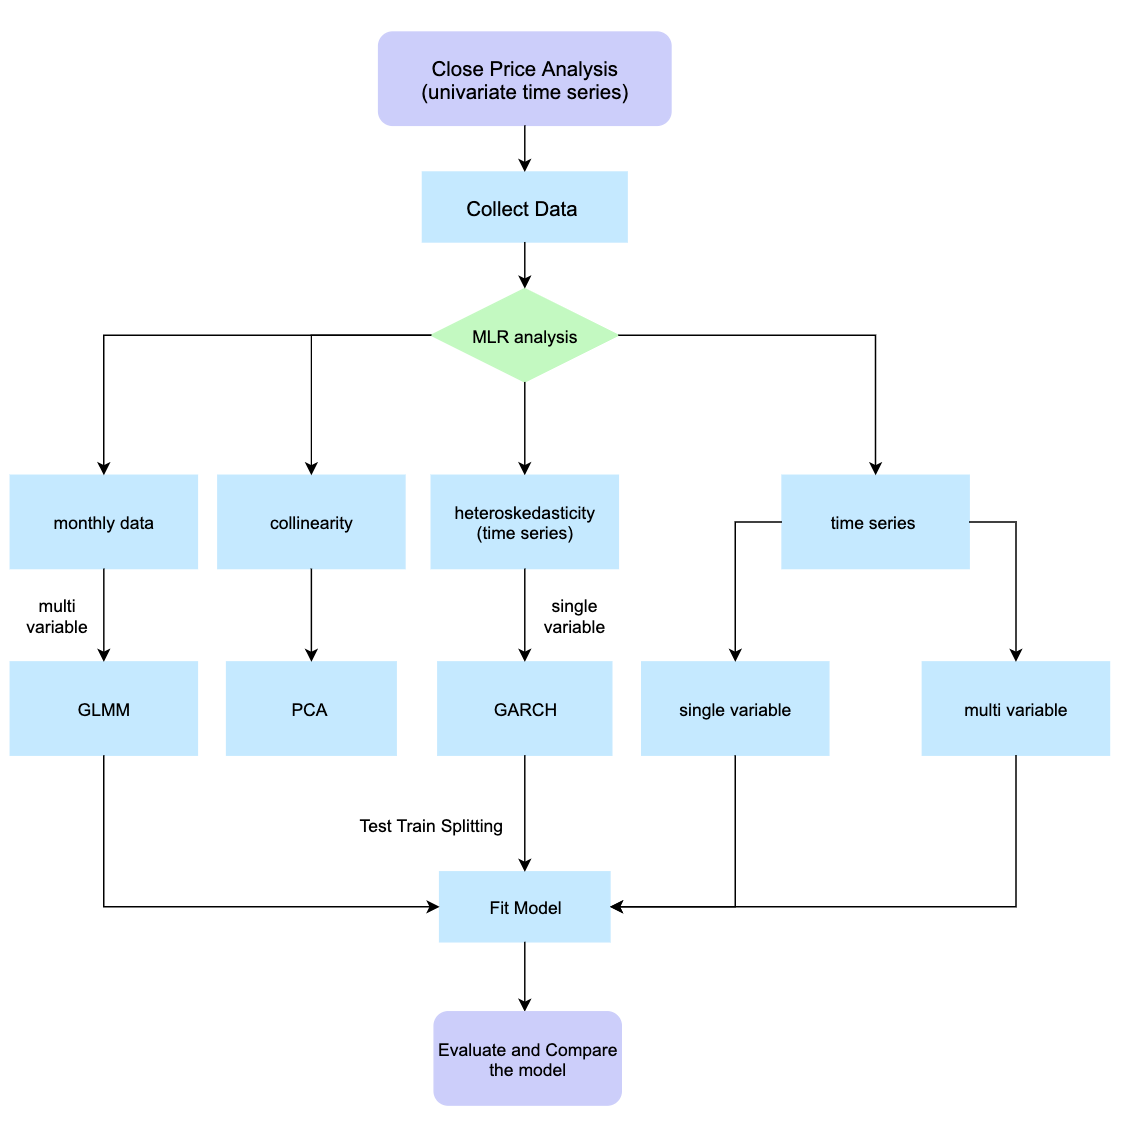
\includegraphics[width=22cm]{proce.png}
\captionof{figure}{\color{NavyBlue} Fit \textit{Close} Flow chart of this project}
\label{flow}
\end{center}
%----------------------------------------------------------------------------------------
%	GEOLOGY
%----------------------------------------------------------------------------------------

\color{Black} % DarkSlateGray color for the rest of the content

\section*{\textit{Close} Price Analysis}
First analyze as a univariate time series.

\begin{center}
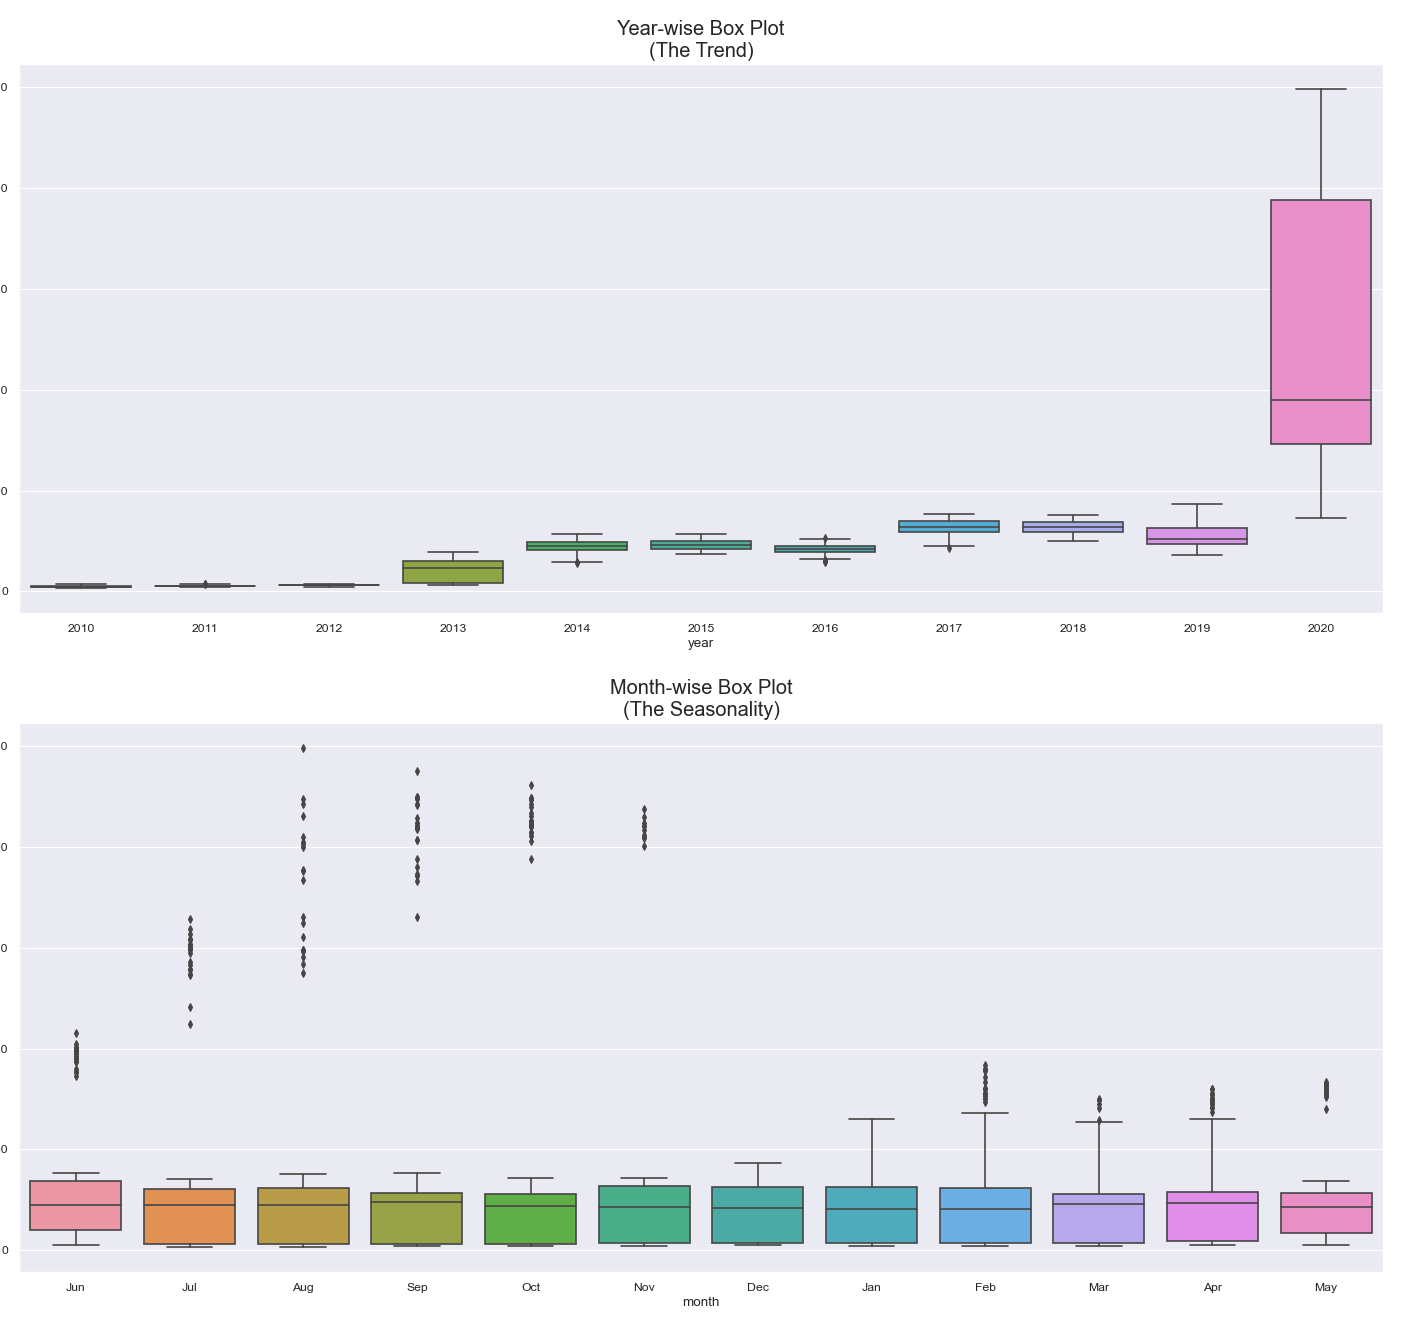
\includegraphics[width=22cm,height=20cm]{x4.png}
\captionof{figure}{\color{NavyBlue} The year-wise and month-wise box plot for potential trend and seasonality. Observe a sharp increase in year 2020 and no obvious seasonality presented. Outliers in the month-wise plot will disappear after fit the same plot with year 2020 data only.}
\end{center}%\vspace{1cm}

\begin{itemize}
    \item As goal is predict $12.7-12.11$ stock price, decide to \textbf{only use year 2020 data}. 
\end{itemize}

\section*{Data Collecting}
The data or variables we used are shown in the table 
\begin{center}
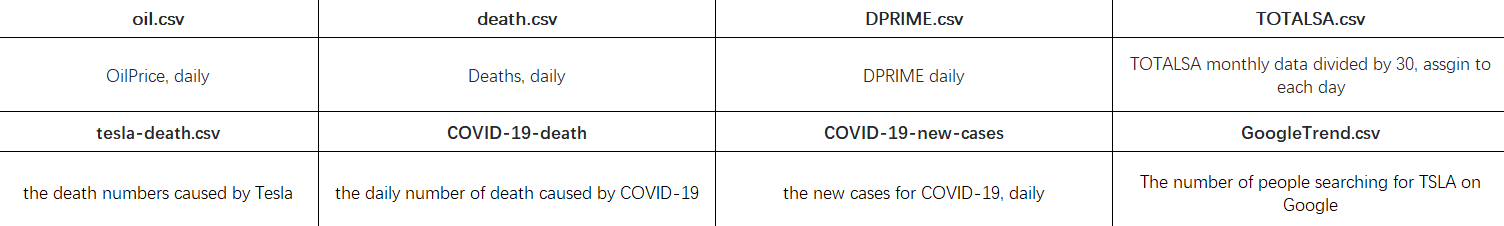
\includegraphics[width=22cm]{vara.png}
\captionof{figure}{\color{NavyBlue} Variable or data we used.}
\end{center}



\subsection*{MLR Analysis}
\textbf{Variable Selection}
\begin{itemize}
\item To find the significant regressors for the multi linear regression, we need to provide the R squared, adjust R Squared, Mallow's Cp, and the BIC for different variable.
\item From the figure, we need to select the variables with dark colors. So it is easy to see that the deaths, new\_deaths, and volume 
are not significant for the linear regression model.
\end{itemize}
\begin{center}\vspace{1cm}
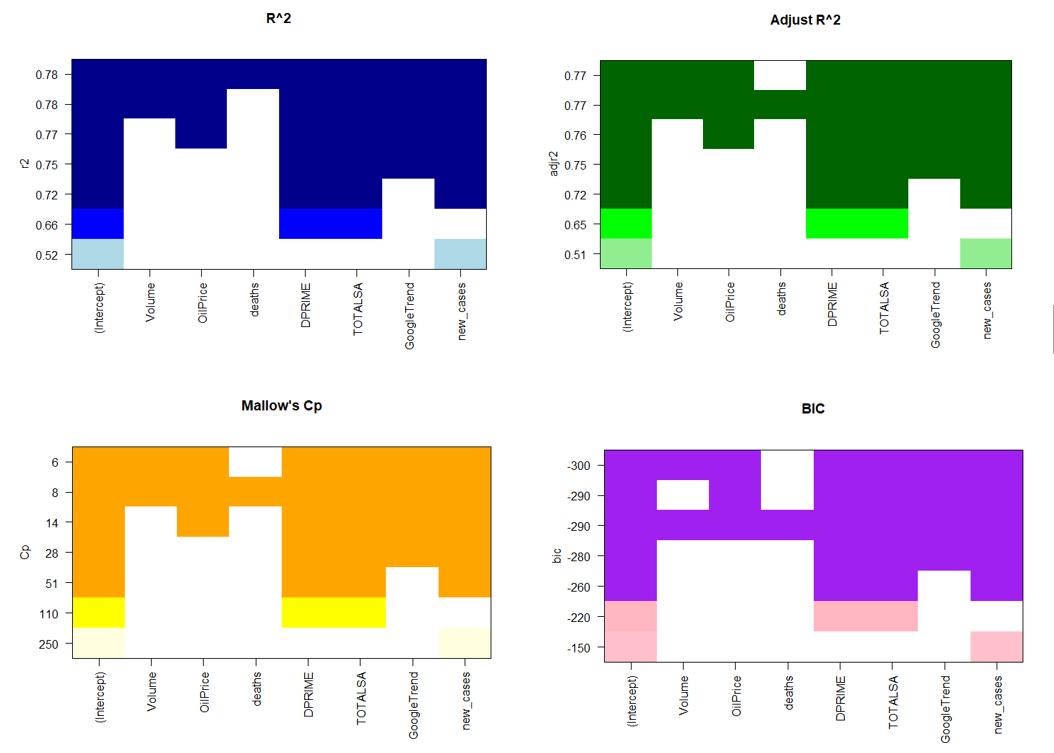
\includegraphics[width=1.0\linewidth]{comb.png}
\captionof{figure}{\color{NavyBlue} output of regsubsets.out plot for different variables to select the significant variable to the model}
\end{center}

\begin{itemize}
    
\item There are some problems in the multi linear model.
\end{itemize}
\begin{center}
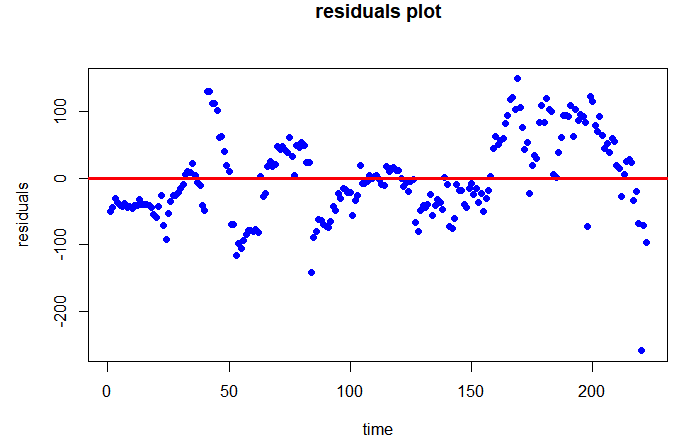
\includegraphics[width=1.0\linewidth]{res.png}
\captionof{figure}{\color{NavyBlue} The residual plot. The variance of residuals increases with the date, and there exists Heteroskedasticity.}
\end{center}
 Moreover, from the acf plot we can see that the errors are highly correlated with each other until the lag around 10, so we also need to analysis the price of the stock as a time series. 
\begin{center}
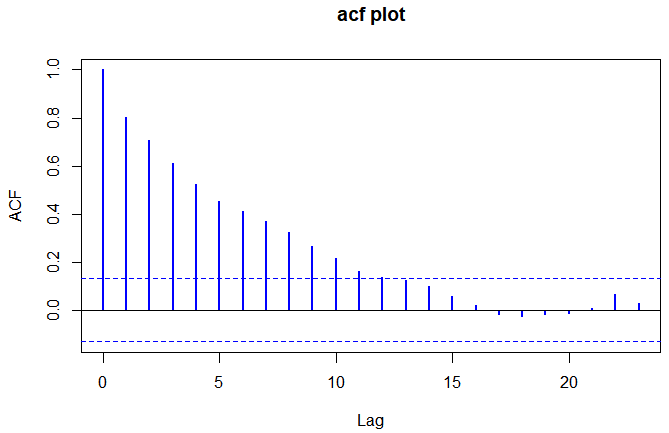
\includegraphics[width=1.0\linewidth]{acf.png}
\captionof{figure}{\color{NavyBlue} Acf plot shows the errors are highly correlated with each other until the lag around 10, the price of the stock should be analyzed as a time series.}
\end{center}


\subsection*{Problem Addressing}
\begin{itemize}
    \item 
For monthly data and heteroskedasticity, GLMM and GARCH are used respectively. No significant influence shown from these metho ds.
\end{itemize}
\subsubsection*{Colinearity}
\begin{center}
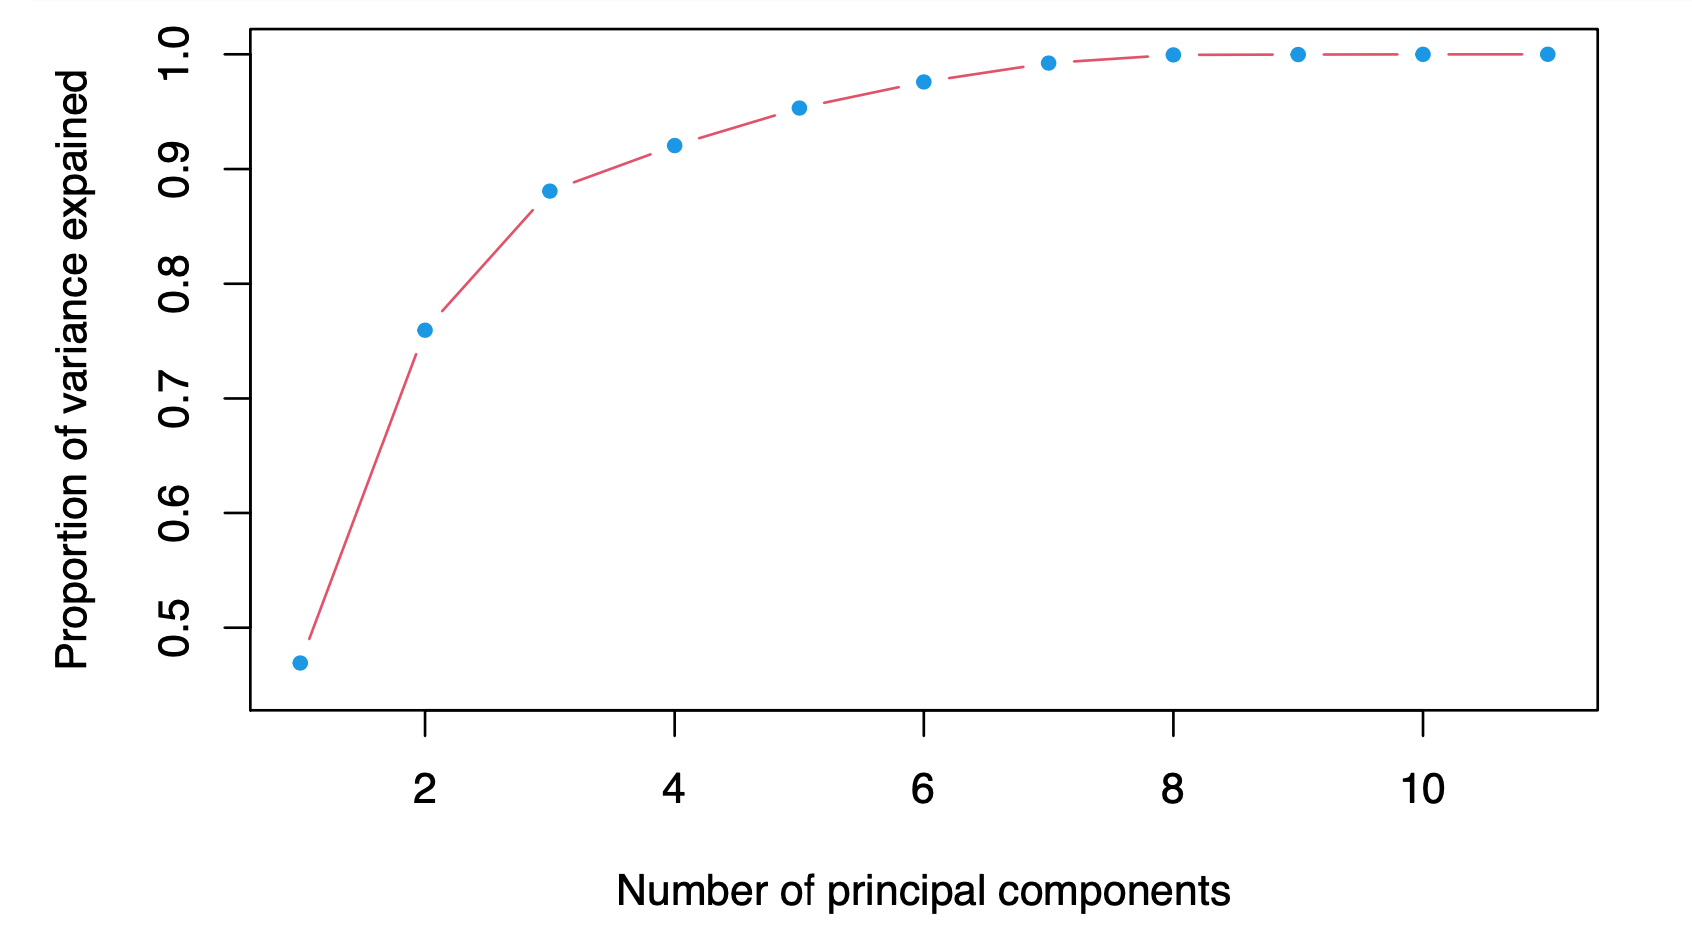
\includegraphics[width=1.0\linewidth]{colli.png}
\captionof{figure}{\color{NavyBlue} he Cumulative Proportion of Variance Explained by Different Principal Component. }
\end{center}
The first four principal components explain over 0.9 of the total variance. Hence we consider the first four components are enough for the model fitting.
\subsubsection*{Time Series}
\begin{itemize}
    \item Single \textit{Close} price model fit, including \textit{simple Exponential Smoothing (SES),Holt’s Method with linear and exponential trend, Holt-Winter expoential trend with addition-addition and addition-multiplication(HWES add-add, HWES add-mul), Seasonal Autoregressive Integrated Moving Average (SARIMA) and autocorrelation(AR)}.
    \item Multiple variable fit. Use \textit{GLMM, ARIMA, Vector-AutoRegression (VAR)} with $4,5,3$ varibales respectively.
    \item All model prediction score are calculated and compared in later section. 
\end{itemize}
% \begin{center}
% \includegraphics[width=1.0\linewidth]{SES.png}
% \captionof{figure}{\color{NavyBlue}Final AR Model Prenset}
% \end{center}\vspace{1cm}

\subsection*{Model Score Comparison}
\begin{itemize}
    \item \textbf{Method}: Train/Test Spilt
    \item \textbf{Criteria}: Predict test set value is $y_{pred}$, original test set $y_{test}$, calculate the score $\sum (y_{pred} - y_{test})^2$. 
\end{itemize}

\begin{center}
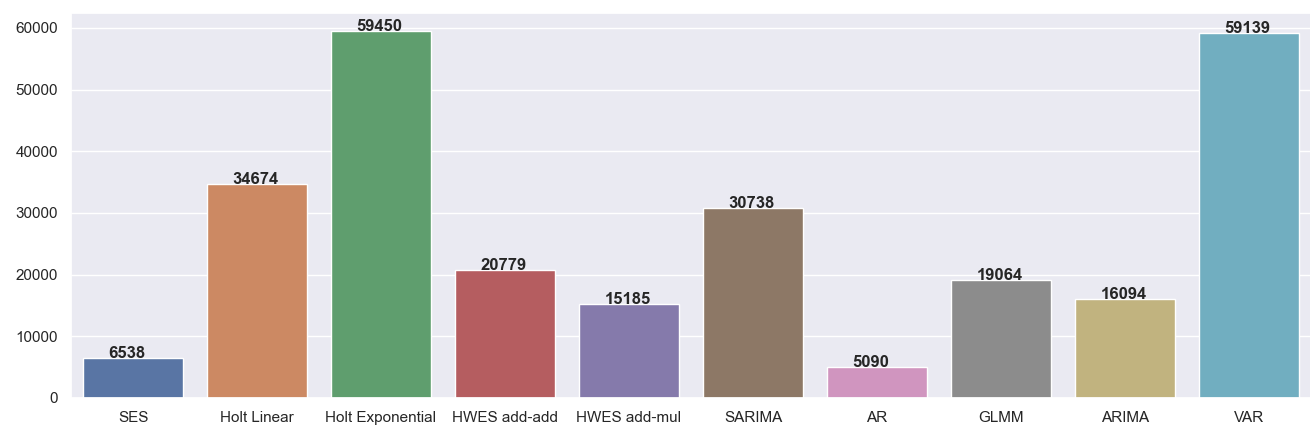
\includegraphics[width=1.0\linewidth]{score.png}
\caption{Test Score for Model}
\captionof{figure}{\color{NavyBlue} Test score for each model. The smaller the score, the better the model is. So choose \textit{AR} model.}
\end{center}\vspace{1cm}
\begin{center}
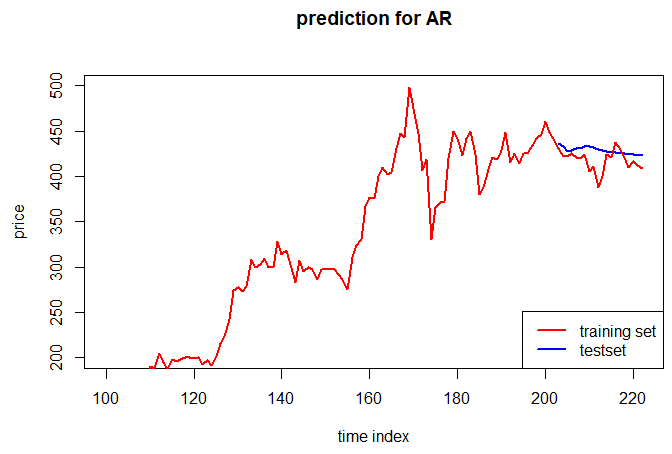
\includegraphics[width=1.0\linewidth]{AR.png}
\captionof{figure}{\color{NavyBlue}Final AR Model Prenset}
\end{center}\vspace{1cm}
%----------------------------------------------------------------------------------------
%	CONCLUSIONS
%----------------------------------------------------------------------------------------

\color{SaddleBrown} % SaddleBrown color for the conclusions to make them stand out

\section*{Conclusions}
We basically find extra parameters that can be used as regressors for stock price prediction. MLR is used to do basic variable selection and problem identifying. We find that there are four problems in total and different methods are used to address them. Then we do predictions of different models on the testing dataset. A bar chart is plotted to compare the residual scores. AR model is finally picked due to its smallest residual sum of squares. Therefore, we use AR model to do the final prediction of stock closing price.
\color{Black} % Set the color back to DarkSlateGray for the rest of the content

%----------------------------------------------------------------------------------------
%	FORTHCOMING RESEARCH
%----------------------------------------------------------------------------------------


\end{multicols}
\end{document}